\subsection{Tower of Hanoi}

Can the above method be used for a degree one recurrence relation?
Remember the Tower of Hanoi problem?
Let $t_n$ be the number of steps to solve the problem.
Recall that we solve the problem by providing
a recursive procedure.
Here's the problem again.
You have $n$ disks that you want to move from A to C.

\begin{console}
12094
\end{console}


We think of the $n$-disk problem in terms of the
$n-1$ disk problem:

\begin{center}
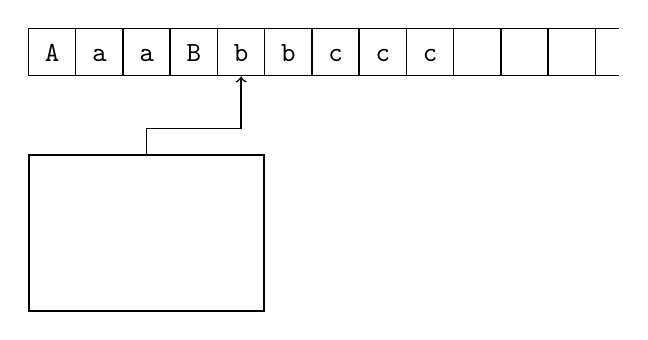
\begin{tikzpicture}

\draw (0.3, 0.3)
  node[draw, line width=0.02cm, , color=black,
       rounded corners=0cm, inner sep=0cm] {

\begin{minipage}[t][0.6cm]{0.6cm}
\mbox{}

\end{minipage}

};\draw (0.3, 0.3) node[color=black] {{\vphantom{AaaBbbccc$\BLANK$$\BLANK$$\BLANK$}\texttt{A}}};
\draw (0.8999999999999999, 0.3)
  node[draw, line width=0.02cm, , color=black,
       rounded corners=0cm, inner sep=0cm] {

\begin{minipage}[t][0.6cm]{0.6cm}
\mbox{}

\end{minipage}

};\draw (0.8999999999999999, 0.3) node[color=black] {{\vphantom{AaaBbbccc$\BLANK$$\BLANK$$\BLANK$}\texttt{a}}};
\draw (1.5, 0.3)
  node[draw, line width=0.02cm, , color=black,
       rounded corners=0cm, inner sep=0cm] {

\begin{minipage}[t][0.6cm]{0.6cm}
\mbox{}

\end{minipage}

};\draw (1.5, 0.3) node[color=black] {{\vphantom{AaaBbbccc$\BLANK$$\BLANK$$\BLANK$}\texttt{a}}};
\draw (2.0999999999999996, 0.3)
  node[draw, line width=0.02cm, , color=black,
       rounded corners=0cm, inner sep=0cm] {

\begin{minipage}[t][0.6cm]{0.6cm}
\mbox{}

\end{minipage}

};\draw (2.0999999999999996, 0.3) node[color=black] {{\vphantom{AaaBbbccc$\BLANK$$\BLANK$$\BLANK$}\texttt{B}}};
\draw (2.7, 0.3)
  node[draw, line width=0.02cm, , color=black,
       rounded corners=0cm, inner sep=0cm] {

\begin{minipage}[t][0.6cm]{0.6cm}
\mbox{}

\end{minipage}

};\draw (2.7, 0.3) node[color=black] {{\vphantom{AaaBbbccc$\BLANK$$\BLANK$$\BLANK$}\texttt{b}}};
\draw (3.3, 0.3)
  node[draw, line width=0.02cm, , color=black,
       rounded corners=0cm, inner sep=0cm] {

\begin{minipage}[t][0.6cm]{0.6cm}
\mbox{}

\end{minipage}

};\draw (3.3, 0.3) node[color=black] {{\vphantom{AaaBbbccc$\BLANK$$\BLANK$$\BLANK$}\texttt{b}}};
\draw (3.9000000000000004, 0.3)
  node[draw, line width=0.02cm, , color=black,
       rounded corners=0cm, inner sep=0cm] {

\begin{minipage}[t][0.6cm]{0.6cm}
\mbox{}

\end{minipage}

};\draw (3.9000000000000004, 0.3) node[color=black] {{\vphantom{AaaBbbccc$\BLANK$$\BLANK$$\BLANK$}\texttt{c}}};
\draw (4.5, 0.3)
  node[draw, line width=0.02cm, , color=black,
       rounded corners=0cm, inner sep=0cm] {

\begin{minipage}[t][0.6cm]{0.6cm}
\mbox{}

\end{minipage}

};\draw (4.5, 0.3) node[color=black] {{\vphantom{AaaBbbccc$\BLANK$$\BLANK$$\BLANK$}\texttt{c}}};
\draw (5.1, 0.3)
  node[draw, line width=0.02cm, , color=black,
       rounded corners=0cm, inner sep=0cm] {

\begin{minipage}[t][0.6cm]{0.6cm}
\mbox{}

\end{minipage}

};\draw (5.1, 0.3) node[color=black] {{\vphantom{AaaBbbccc$\BLANK$$\BLANK$$\BLANK$}\texttt{c}}};
\draw (5.699999999999999, 0.3)
  node[draw, line width=0.02cm, , color=black,
       rounded corners=0cm, inner sep=0cm] {

\begin{minipage}[t][0.6cm]{0.6cm}
\mbox{}

\end{minipage}

};\draw (5.699999999999999, 0.3) node[color=black] {{\vphantom{AaaBbbccc$\BLANK$$\BLANK$$\BLANK$}\texttt{$\BLANK$}}};
\draw (6.299999999999999, 0.3)
  node[draw, line width=0.02cm, , color=black,
       rounded corners=0cm, inner sep=0cm] {

\begin{minipage}[t][0.6cm]{0.6cm}
\mbox{}

\end{minipage}

};\draw (6.299999999999999, 0.3) node[color=black] {{\vphantom{AaaBbbccc$\BLANK$$\BLANK$$\BLANK$}\texttt{$\BLANK$}}};
\draw (6.899999999999999, 0.3)
  node[draw, line width=0.02cm, , color=black,
       rounded corners=0cm, inner sep=0cm] {

\begin{minipage}[t][0.6cm]{0.6cm}
\mbox{}

\end{minipage}

};\draw (6.899999999999999, 0.3) node[color=black] {{\vphantom{AaaBbbccc$\BLANK$$\BLANK$$\BLANK$}\texttt{$\BLANK$}}};\draw[line width=0.02cm,black] (7.1999999999999975,0.6) to  (7.499999999999998,0.6);
\draw[line width=0.02cm,black] (7.1999999999999975,0.0) to  (7.499999999999998,0.0);

\draw (1.5, -2.0)
  node[draw, line width=0.02cm, , color=black,
       rounded corners=0cm, inner sep=0cm] {

\begin{minipage}[t][1.98cm]{2.98cm}
\mbox{}

\end{minipage}

};\draw[line width=0.02cm,black,->] (1.5,-1) to  (1.5,-0.67) to  (2.7,-0.67) to  (2.7,-0.01);
\end{tikzpicture}

\end{center}



We ignore disk $n$ for the time being
and apply our procedure to move the top $n-1$ disks from A to B:

%-*-latex-*-
\begin{Verbatim}[frame=single,fontsize=\small]
[student@localhost discrete-probability] python discrete-probrobability/game2.py
python: can't open file 'discrete-probrobability/game2.py': [Errno 2] No such fi
le or directory
\end{Verbatim}



This should take $t_{n-1}$ steps.
Now we move disk $n$ from A to C:

\begin{center}
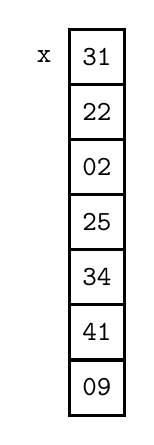
\begin{tikzpicture}

\draw (0.35, -0.35)
  node[draw, line width=0.04cm, , color=black,
       rounded corners=0cm, inner sep=0cm] {

\begin{minipage}[t][0.7cm]{0.7cm}
\mbox{}

\end{minipage}

};\draw (0.35, -0.35) node[color=black] {{\texttt{31}}};
\draw (0.35, -1.0499999999999998)
  node[draw, line width=0.04cm, , color=black,
       rounded corners=0cm, inner sep=0cm] {

\begin{minipage}[t][0.7cm]{0.7cm}
\mbox{}

\end{minipage}

};\draw (0.35, -1.0499999999999998) node[color=black] {{\texttt{22}}};
\draw (0.35, -1.7499999999999996)
  node[draw, line width=0.04cm, , color=black,
       rounded corners=0cm, inner sep=0cm] {

\begin{minipage}[t][0.7cm]{0.7cm}
\mbox{}

\end{minipage}

};\draw (0.35, -1.7499999999999996) node[color=black] {{\texttt{02}}};
\draw (0.35, -2.4499999999999997)
  node[draw, line width=0.04cm, , color=black,
       rounded corners=0cm, inner sep=0cm] {

\begin{minipage}[t][0.7cm]{0.7cm}
\mbox{}

\end{minipage}

};\draw (0.35, -2.4499999999999997) node[color=black] {{\texttt{25}}};
\draw (0.35, -3.15)
  node[draw, line width=0.04cm, , color=black,
       rounded corners=0cm, inner sep=0cm] {

\begin{minipage}[t][0.7cm]{0.7cm}
\mbox{}

\end{minipage}

};\draw (0.35, -3.15) node[color=black] {{\texttt{34}}};
\draw (0.35, -3.8499999999999996)
  node[draw, line width=0.04cm, , color=black,
       rounded corners=0cm, inner sep=0cm] {

\begin{minipage}[t][0.7cm]{0.7cm}
\mbox{}

\end{minipage}

};\draw (0.35, -3.8499999999999996) node[color=black] {{\texttt{41}}};
\draw (0.35, -4.550000000000001)
  node[draw, line width=0.04cm, , color=black,
       rounded corners=0cm, inner sep=0cm] {

\begin{minipage}[t][0.7cm]{0.7cm}
\mbox{}

\end{minipage}

};\draw (0.35, -4.550000000000001) node[color=black] {{\texttt{09}}};
\draw (-0.32, -0.35)
  node[draw=none, line width=0cm, , color=black,
       rounded corners=0cm, inner sep=0cm] {

\begin{minipage}[t][0.1cm]{0.1cm}
\mbox{}

\end{minipage}

};\draw (-0.32, -0.35) node[color=black] {\text{\texttt{x}}};
\end{tikzpicture}

\end{center}



That takes 1 step.
And finally we apply our procedure to move
the $n-1$ disks from $B$ to $C$:

\begin{console}[frame=single, , commandchars=~@$]
SLNode * p = phead;
while (p != NULL)
{
    std::cout << (*p) << std::endl;
    p = p->next();
}
\end{console}

and the output is this:
\begin{console}[frame=single,fontsize=\footnotesize]
[student@localhost linkedlist] g++ tmp12345678.cpp; ./a.out
<SLNode 0x7ffcf03deca0 key:2, next:0x7ffcf03decb0>
<SLNode 0x7ffcf03decb0 key:6, next:0x7ffcf03decc0>
<SLNode 0x7ffcf03decc0 key:4, next:0x7ffcf03decd0>
<SLNode 0x7ffcf03decd0 key:5, next:0>
\end{console}



That takes $t_{n-1}$ steps.
Altogther we took $t_{n-1} + 1 + t_{n-1}$ steps.
Hence
\begin{align*}
t_n 
&= t_{n-1} + 1 + t_{n-1} \\
&= 2 t_{n-1} + 1
\end{align*}
We need a base condition.
So what's $t_0$?
That's the problem with $0$ disks.
It should probably be 0 step: $t_0 = 0$.
But vacuous problems are sometimes dangeourous.
So let's consider $t_1$.
Clearly $t_1 = 1$.
Now since we want $t_1 = 2t_0 + 1$, we have
\[
1 = 2 t_0 + 1
\]
and, yes, we do get $t_0 = 0$.
Altogether we have
\[
t_n = 
\begin{cases}
0 &\text{ if } n = 0 \\
2 t_{n-1} + 1 &\text{ if } n > 0
\end{cases}
\]
Furthermore note that the recurrence relation is not just defined
in terms of a linear combination of $t_n$'s for small $n$:
There's a \lq\lq + 1'' in the recurrence relation:
\[
t_n = 2 t_{n-1} \underline{ + 1 }
\]
This is a degree 1 nonhomogeneous recurrence relation.

For this recurrence relation, it's so simple that you can
actually find a closed form quickly, using \lq\lq substitutions".
Here's how you would do it.
\begin{align*}
t_n
&= 2 t_{n-1} + 1 \\ 
&= 2 ( 2t_{n-2} + 1) + 1 = 4t_{n-2} + 2 + 1 \\ 
&= 4 (2 t_{n-3} + 1 ) + 2 + 1 = 8 t_{n-3} + 4 + 2 + 1
\end{align*}
All the above assume that $n \geq 3$.
At this point you see a pattern:
\begin{align*}
t_n
&= 2^3 t_{n-3} + 2^2 + 2^1 + 2^0
\end{align*}
To check on the pattern, you do one more step (assuming $n \geq 4$):
\begin{align*}
t_n
&= 2^3 t_{n-3} + 2^2 + 2^1 + 2^0 \\ 
&= 2^3 (2t_{n-4} + 1) + 2^2 + 2^1 + 2^0 = 2^4t_{n-4} + 2^3 + 2^2 + 2^1 + 2^0
\end{align*}
i.e.,
\begin{align*}
t_n
&= 2^3 t_{n-3} + 2^2 + 2^1 + 2^0 \\ 
&= 2^4t_{n-4} + 2^3 + 2^2 + 2^1 + 2^0 \\
&= ... \\
&= 2^kt_{n-k} + 2^{k-1} + 2^{k-2} + \cdots + 2^3 + 2^2 + 2^1 + 2^0
\end{align*}
At some point you'd reach the base case, i.e., when $n - k = 1$,
\begin{align*}
t_n
&= 2^{n-1}t_{1} + 2^{n-2} + 2^{n-3} + \cdots + 2^3 + 2^2 + 2^1 + 2^0 \\
&= 2^{n-1} + 2^{n-2} + 2^{n-3} + \cdots + 2^3 + 2^2 + 2^1 + 2^0 \\
&= 2^n - 1
\end{align*}
by the geometric sum formula.
TADA!

So immediately, you know that to solve the tower of hanoi problem
you need to make $2^{32} - 1 = 4294967295$ move.

Now to be absolutely mathematically correct, the following
from the above:
\begin{align*}
t_n
&= 2^3 t_{n-3} + 2^2 + 2^1 + 2^0 \\ 
&= 2^4t_{n-4} + 2^3 + 2^2 + 2^1 + 2^0 \\
&= ... \\
&= 2^kt_{n-k} + 2^{k-1} + 2^{k-2} + \cdots + 2^3 + 2^2 + 2^1 + 2^0
\end{align*}
is not absolutely rigorous.
Why? Because it this:
\begin{align*}
t_n
&= ... (\leftarrow \text{look at the missing steps described by \lq\lq ..."}) \\ 
&= 2^kt_{n-k} + 2^{k-1} + 2^{k-2} + \cdots + 2^3 + 2^2 + 2^1 + 2^0
\end{align*}
The above leads to
\[
t_n = 2^n - 1
\]
Generally, this is what will happen in the mathematical derivation
of 
$t_n = 2^n - 1$.
The above is OK, as long as it is to derive a plausible closed form for $t_n$.
After that you prove $t_n = 2^n - 1$ is indeed true by induction, using the recurrence relation.


\begin{ex} 
  \label{ex:some-decision1}
  \tinysidebar{\debug{exercises/{empty0/question.tex}}}
  \solutionlink{sol:some-decision1}
  \qed
\end{ex} 
\begin{python0}
from solutions import *
add(label="ex:some-decision1",
    srcfilename='exercises/some-decision1/answer.tex') 
\end{python0}


\newpage
Another thing to note is this very importact fact:

\begin{longtable}{|r||r|r|r|r|r|}
\hline 
         & $0$ & $1$ & $2$ & $3$ & $\ldots$ \\ \hline \hline 
$x_0$    & 5   & 0   & 0   & 0   & ...      \\ \hline 
$x_1$    & 1   & 4   & 1   & 5   & ...      \\ \hline 
$x_2$    &     &     &     &     &          \\ \hline 
$x_3$    &     &     &     &     &          \\ \hline 
$\ldots$ &     &     &     &     &          \\ \hline 
\end{longtable}
        



\begin{ex} 
  \label{ex:some-decision1}
  \tinysidebar{\debug{exercises/{empty0/question.tex}}}
  \solutionlink{sol:some-decision1}
  \qed
\end{ex} 
\begin{python0}
from solutions import *
add(label="ex:some-decision1",
    srcfilename='exercises/some-decision1/answer.tex') 
\end{python0}


\newpage\myinput{tower-of-hanoi-variations.tex}


\begin{ex} 
  \label{ex:some-decision1}
  \tinysidebar{\debug{exercises/{empty0/question.tex}}}
  \solutionlink{sol:some-decision1}
  \qed
\end{ex} 
\begin{python0}
from solutions import *
add(label="ex:some-decision1",
    srcfilename='exercises/some-decision1/answer.tex') 
\end{python0}



\begin{ex} 
  \label{ex:some-decision1}
  \tinysidebar{\debug{exercises/{empty0/question.tex}}}
  \solutionlink{sol:some-decision1}
  \qed
\end{ex} 
\begin{python0}
from solutions import *
add(label="ex:some-decision1",
    srcfilename='exercises/some-decision1/answer.tex') 
\end{python0}



\begin{ex} 
  \label{ex:some-decision1}
  \tinysidebar{\debug{exercises/{empty0/question.tex}}}
  \solutionlink{sol:some-decision1}
  \qed
\end{ex} 
\begin{python0}
from solutions import *
add(label="ex:some-decision1",
    srcfilename='exercises/some-decision1/answer.tex') 
\end{python0}



\begin{ex} 
  \label{ex:some-decision1}
  \tinysidebar{\debug{exercises/{empty0/question.tex}}}
  \solutionlink{sol:some-decision1}
  \qed
\end{ex} 
\begin{python0}
from solutions import *
add(label="ex:some-decision1",
    srcfilename='exercises/some-decision1/answer.tex') 
\end{python0}



\begin{ex} 
  \label{ex:some-decision1}
  \tinysidebar{\debug{exercises/{empty0/question.tex}}}
  \solutionlink{sol:some-decision1}
  \qed
\end{ex} 
\begin{python0}
from solutions import *
add(label="ex:some-decision1",
    srcfilename='exercises/some-decision1/answer.tex') 
\end{python0}



\begin{ex} 
  \label{ex:some-decision1}
  \tinysidebar{\debug{exercises/{empty0/question.tex}}}
  \solutionlink{sol:some-decision1}
  \qed
\end{ex} 
\begin{python0}
from solutions import *
add(label="ex:some-decision1",
    srcfilename='exercises/some-decision1/answer.tex') 
\end{python0}


\myinput{tower-of-hanoi-generating-function.tex}
